\clearpage
\section{Datasets Proposed in the Scientific Literature}
The works whose main contribution is the 
creation of a dataset are mostly preprints, 
and thus require careful consideration. 
The papers primarily dedicated to dataset 
generation include: CoDet-M4 \cite{orel2025codet}, 
AIGCodeSet \cite{demirok2024aigcodeset}, 
and CodeMirage \cite{guo2025codemirage}.

\subsection*{CoDet-M4}
The main contribution of this work is the construction 
of a dataset derived from existing human-written code datasets, 
by generating synthetic code using six different LLMs. 
The authors then train several models on this dataset 
to evaluate their performance, 
demonstrating that their dataset can significantly improve 
the effectiveness of various code detection models.
The authors employ the following models as code generators:

\begin{itemize}
    \item \textbf{GPT-4o}: A proprietary model developed by OpenAI, selected to represent the state-of-the-art among large-scale, closed-source LLMs.
    
    \item \textbf{CodeLlama (7B)}: An open-source model by Meta, specifically trained for code-related tasks. It is one of the most popular code-oriented language models.
    
    \item \textbf{Llama3.1 (8B)}: A more recent version of Meta’s Llama family. Although it is a general-purpose model, it exhibits strong performance in code generation.
    
    \item \textbf{CodeQwen 1.5 (7B)}: An open-source model from Alibaba Cloud, also specialized in code, and part of the Qwen series.
    
    \item \textbf{Nxcode-orpo (7B)}: A fine-tuned variant of CodeQwen. The authors include it to evaluate the robustness of detectors against different fine-tuning strategies applied to the same base model (in this case, ORPO – Monolithic Preference Optimization).
\end{itemize}


\subsubsection*{Strengths}
\begin{itemize}
    \item The introduction of one of the most extensive and diverse datasets proposed for the task of LLM-generated code detection.
    \item Dataset cleaning is carefully performed, including the use of \textit{Codeforces} as one of the tools to assess the correctness of human-written code {(\scriptsize\textit{Section 3.3: Quality Assurance})}.
    \item The authors also construct an ``out-of-domain'' dataset, specifically designed to contain code with characteristics intentionally different from the main dataset {(\scriptsize\textit{Section 4.4:Out-of-Domain Experiment})}.
    \item The dataset includes code in three different programming languages, unlike other works that focus solely on Python {(\scriptsize\textit{Section 3.1: Data Collection})}.
\end{itemize}

\subsubsection*{Weaknesses}
\begin{itemize}
    \item Suspiciously high in-domain classification metrics, with F-scores exceeding 98\% {(\scriptsize\textit{Table 2})}.
    \item The prompts used to generate synthetic code vary depending on the source, potentially introducing an unintentional correlation between code types and the generation prompts {(\scriptsize\textit{Appendix F})}.
    \item Most of the LLMs used for code generation are lightweight models, with GPT-4o being the only large-scale LLM involved {(\scriptsize\textit{Section 3.2: Code Generation})}.
\end{itemize}


Once the dataset is downloaded from the \href{https://huggingface.co/datasets/DaniilOr/CoDET-M4}{official portal}, 
several important features are found to be missing:
\begin{enumerate}
    \item The declared train/validation/test split described in the paper is not included; only the test set is provided. This makes \textbf{reproducing their results more difficult}.
    \item Some significant \textbf{code-level features are missing}, such as whether the code sample is class-based or function-based.
    \item The authors state in the paper that they plan to keep updating the dataset, which may explain small discrepancies in the number of code samples compared to what is reported. For example, there are fewer GitHub samples than those claimed in the original publication.
\end{enumerate}


\begin{figure}[H]
    \centering
    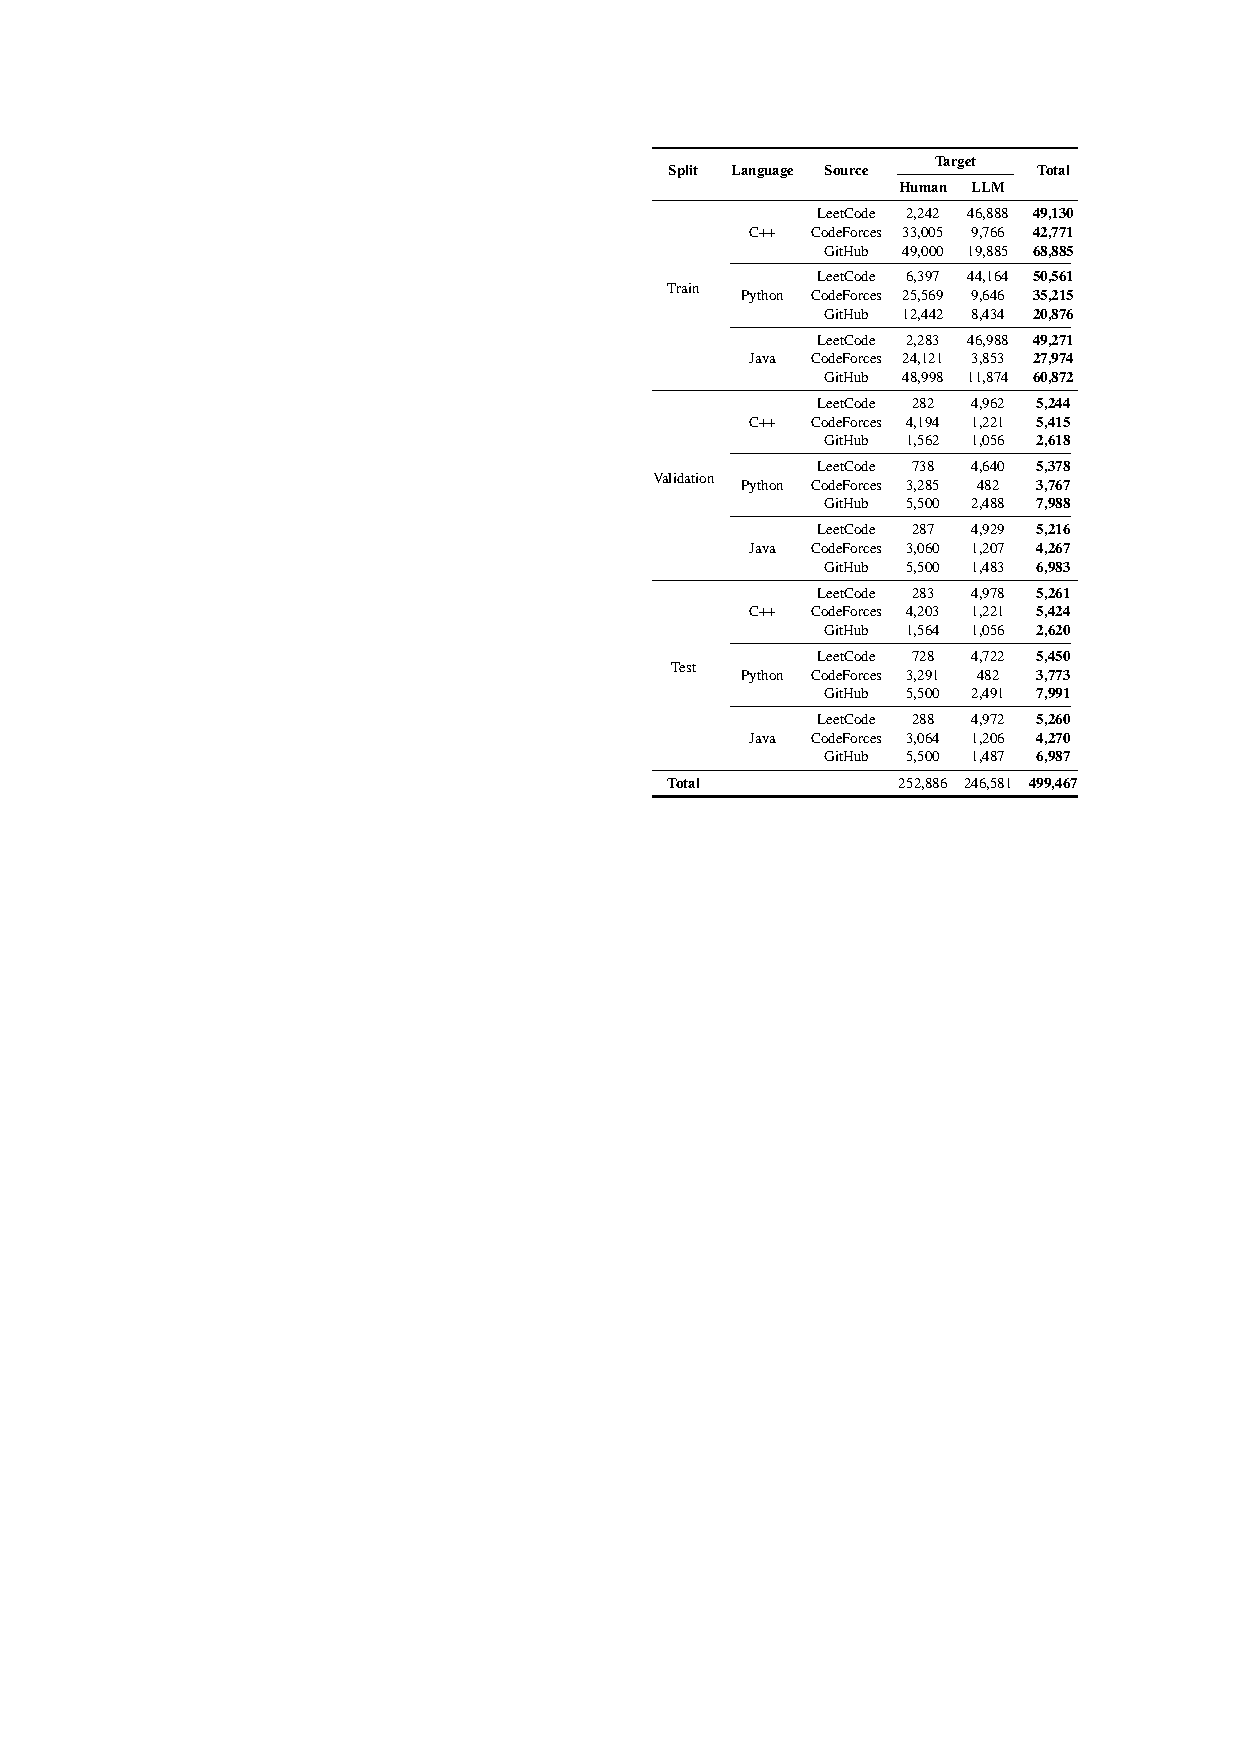
\includegraphics[width=0.5\textwidth]{img/CoDet-M4/tab1.pdf} % Inserisci il nome corretto del file immagine
    \caption{Table 1 \cite{orel2025codet}: Number of code snippets in train/val/test sets}
    \label{fig:table1_CoDet-M4}
\end{figure}
